% Тут используется класс, установленный на сервере Papeeria. На случай, если
% текст понадобится редактировать где-то в другом месте, рядом лежит файл matmex-diploma-custom.cls
% который в момент своего создания был идентичен классу, установленному на сервере.
% Для того, чтобы им воспользоваться, замените matmex-diploma на matmex-diploma-custom
% Если вы работаете исключительно в Papeeria то мы настоятельно рекомендуем пользоваться
% классом matmex-diploma, поскольку он будет автоматически обновляться по мере внесения корректив
%
\documentclass{matmex-diploma}
\usepackage{listings}
\newfontfamily\cyrillicfonttt{CMU Serif}

\lstdefinelanguage{FSharp}%
{morekeywords={let, new, match, with, rec, open, module, namespace, type, of, member, % 
and, for, while, true, false, in, do, begin, end, fun, function, return, yield, try, %
mutable, if, then, else, cloud, async, static, use, abstract, interface, inherit, finally },
  otherkeywords={ let!, return!, do!, yield!, use!, var, from, select, where, order, by },
  keywordstyle=\color{bluekeywords},
  sensitive=true,
  basicstyle=\ttfamily,
	breaklines=true,
  xleftmargin=\parindent,
  aboveskip=\bigskipamount,
	tabsize=4,
  morecomment=[l][\color{greencomments}]{///},
  morecomment=[l][\color{greencomments}]{//},
  morecomment=[s][\color{greencomments}]{{(*}{*)}},
  morestring=[b]",
  showstringspaces=false,
  literate={`}{\`}1,
  stringstyle=\color{redstrings},
}
\lstset{
basicstyle=\small,
identifierstyle=\ttfamily,
keywordstyle=\bfseries,
commentstyle=\scriptsize\rmfamily,
basewidth={0.5em,0.5em},
fontadjust=true,
escapechar=~,
language=haskell
}

\begin{document}
% Год, город, название университета и факультета предопределены,
% но можно и поменять.
% Если англоязычная титульная страница не нужна, то ее можно просто удалить.
\filltitle{ru}{
    chair              = {Кафедра Системного Программирования},
    title              = {Реализация полиномиальной сложности оптимальных принтер-комбинаторов с выбором на платформе .NET},
    type               = {coursework},
    position           = {студента},
    group              = 242,
    author             = {Булгаков Андрей Вадимович},
    supervisorPosition = {ст. преп.},
    supervisor         = {Григорьев С.\,В.},
%    reviewerPosition   = {ст. преп.},
  %  reviewer           = {Григорьев С.\,В.},
%    chairHeadPosition  = {д.\,ф.-м.\,н., профессор},
 %   chairHead          = {Хунта К.\,Х.},
   university         = {Санкт-Петербургский Государственный Университет},
   faculty            = {Математико-механический факультет},
   city               = {Санкт-Петербург},
   year               = {2013}
}
\maketitle
\tableofcontents
\section*{Введение}
При разработке программного обеспечения важную роль играет этап поддержки. Понимание кода проекта на этом этапе занимает особую роль. Неаккуратное оформление программного текста может быть существенным недостатком при работе с ним и вызывать затруднения понимания структуры кода. В большинстве языков для компилятора нет разницы в красиво отформатированном коде т.к. ему нужна синтаксическая и семантическая правильность. В то время как разработчику важно, чтобы код был еще хорошо структурирован и оформлен.
    В дальнейшем языком, с которым мы будем работать является абстрактный язык L.
L состоит из:
\begin{itemize}
    \item констант
    \item переменных
    \item бинарных операций
\end{itemize}
Также в L имеются следующие операторы
\begin{itemize}
    \item присваивание
    \item ветвление
    \item чтение в переменную
    \item вывод переменной
    \item цикл с предусловием
\end{itemize}
Рассмотрим пример двух одинаковых с точки зрения компилятора фрагметов кода на языке L
\begin{figure}[h]
    \centering
    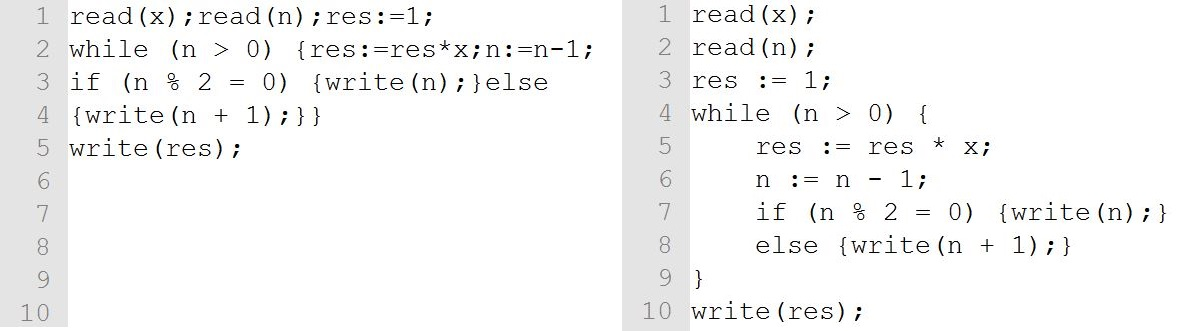
\includegraphics[scale=0.5]{Images/image01.png}
    \caption{Вариант1,Вариант2}
\end{figure}
\\Легко видеть, что вариант 1 труднее для понимания человеком чем вариант 2. Процесс преобразования неформатированного кода в форматированный называется  pretty printing, а инструмент вывода принтером.

Можно сформулировать следующие требования для принтера:
\begin{itemize}
    \item Синтаксическая и семантическая правильность вывода 
    \item Вывод согласно установленным критериям качества оформления
\end{itemize}

Задача построения абстрактного синтаксического дерева для дальнейшего использования принтером и контроля результата его работы ложится на языковые процессоры. Языковые процессоры(ЯП) — это программное средство, принимающее не вход программу в виде текста на некотором языке и решающее определённую задачу над этой программой. К языковым процессорам можно отнести: компиляторы, суперкомпиляторы, интерпретаторы, средства статического анализа кода, интегрированные средства разработки(IDE) и др.

Но как формализовать критерии качества оформления кода?  Для решения этой задачи следует использовать добавление и удаление символов не несущих информации для синтаксического анализа, а также дополнительное ограничения на ширину вывода принтера.

Дополнительной сложностью будет то, что в большинстве случаев нельзя единственным образом сопоставить синтаксическую конструкцию вывода соответствующего данной ширине. Рассмотрим уже использовавшийся пример неформатированного кода. Если вывести представления, соответствующие ширине 35, то помимо варианта 2 возможны следующие представления форматированного кода.
\begin{figure}[h]
    \centering
    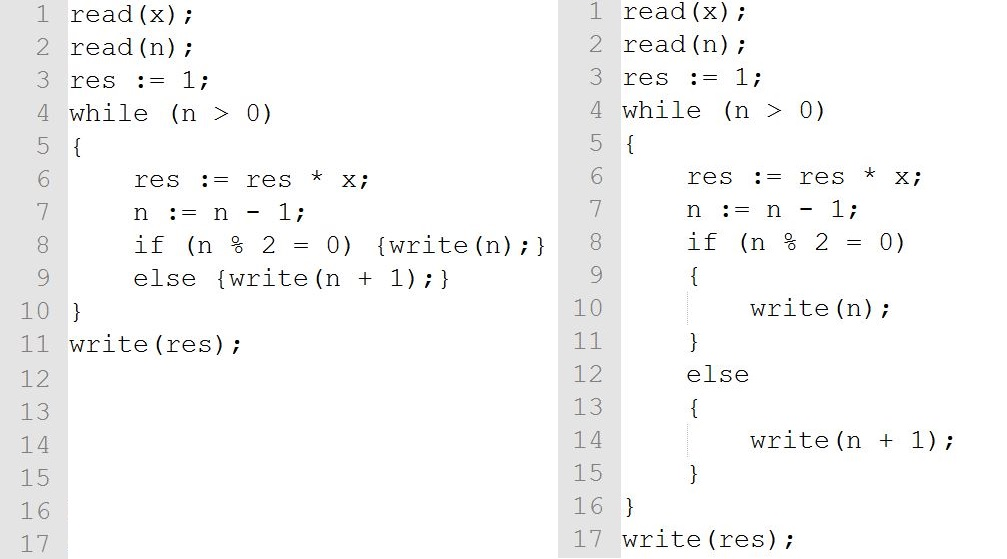
\includegraphics[scale=0.5]{Images/image08.png}
    \caption{Вариант3,Вариант4}
\end{figure}
\\Следовательно нужно ввести дополнительный критерий позволяющий выбрать наиболее \textbf{оптимальный} вариант. Таким критерием будет высота(минимальное число строк) текста, так как он улучшит обозримость вывода. 

Таким образом сформулируем окончательные критерии оптимального принтера:
\begin{itemize}
    \item Синтаксическая и семантическая правильность отформатированного кода
    \item Вывод по возможности не превышающий установленной ширины
    \item Вывод содержащий минимальное количество строк из всевозможных вариантов скомбинированных блоков.
\end{itemize}
Способом задания принтеров обычно являются принтер-комбинаторы.~\cite{podkopaevD, podkopaevR, printComb}
Целью данной работы является разработка библиотеки принтер-комбинаторов на основе работы~\cite{podkopaevD}, предназначенной для использования при создании принтеров.
\section{Обзор}
\subsection{Основные принципы}
Основными принципом построения вывода текста является возможность строить схемы взаимодействия текста и затем представлять его в виде блоков. В большинстве библиотек для этого задается основной тип, который в дальнейшем будет называться документом. Документ предоставляет собой структуру описывающую множество возможных раскладок блоков текста относительно друг друга. Операции, осуществляемые над документами, называются комбинаторами.~\cite{ podkopaevR}
Рассмотрим основные способы расположения текста:
\begin{figure}[h]
    \centering
    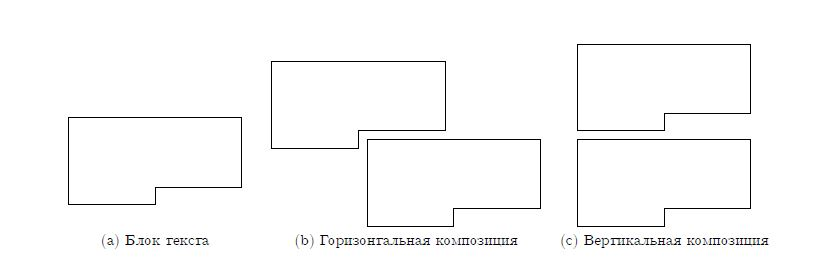
\includegraphics[scale=0.7]{Images/image10.png}
    \caption{Способы расположения}
\end{figure}
\\Варианты (b) и (с) в дальнейшем будем называть Beside и Above
Так же для корректной работы принтера необходим комбинатор выбора между горизонтальной или вертикальной композиции для конкретных документов (далее Choice). Иначе говоря, choice является объединением множеств раскаладок переданных как аргументы документов. Для задания отступов добавим соответствующий комбинатор, который будет называться indent.

Рассмотрим некоторые существующие библиотеки и их отличия
\subsection{Существующие аналоги}
\subsubsection{Polynomial Pretty Printer Combinators}
Написана на языке Haskell позволяет комбинировать и выводить текстовые блоки. Типом задающим множество раскладок блоков и  алгебру комбинаторов здесь является Doc.
\begin{lstlisting}
data Doc = Text String
         | Indent Int Doc
         | Doc `Beside` Doc
         | Doc `Above`  Doc
         | Doc `Choice` Doc
\end{lstlisting}
Документ конструируется с помощью следующих комбинаторов, который аналогичны описанным ранее операциям построения блоков текста.
\begin{lstlisting}
text    :: String -> Doc
indent  :: Int -> Doc -> Doc
beside  :: Doc -> Doc -> Doc
above   :: Doc -> Doc -> Doc
choice  :: Doc-> Doc -> Doc
\end{lstlisting}
После обработки алгоритмом принтера Doc переводится в множество вариантов скомбинированного текста прямоугольной формы. Каждый такой вариант представлен типом Format.
\begin{lstlisting}
data Format = Elem { height  :: Int
                   , last_w  :: Int
                   , total_w :: Int
                   , txtstr  :: Int -> String -> String
                   }
\end{lstlisting}
Он определяет геометрические размеры блока(высоту, ширину, высоту последней строчки), а также функцию преобразования блока в текст.  С помощью данных параметров и выполняется поиск наиболее оптимального блока. Очевидно, что наличие множества обуславливается комбинатором ветвления choice в типе Doc. При этом  каждый сгенерированный Format является линейной структурой.
\begin{figure}[h]
    \centering
    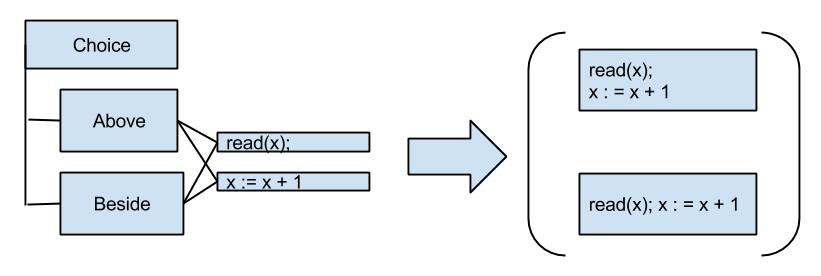
\includegraphics[scale=0.7]{Images/image15.png}
    \caption{Способы расположения}
\end{figure}
\\Множество объектов типа Format реализуется в виде ассоциативного массива, где ключом каждого элемента выступает объект типа Frame, описывающий ширины соответствующего ему Format. При добавлении элементов в этот массив каждой паре (key, value) сопоставляется минимальный по числу строк блок текста. Таким образом на завершающем этапе алгоритма из данного массива выбирается элемент с минимальным значением числа строк, что обеспечивает оптимальность принтера. 
Алгоритм удовлетворяет сформулированным критериям оптимального принтера и именно поэтому он был выбран для создания нашей библиотеки.
Подробнее библиотека с дальнейшей её реализацией на языке Kotlin описана в~\cite{podkopaevD}.
\subsubsection{FSharpx.Text.StructuredFormat}
Библиотека StructuredFormat написанная на языке F\# позволяет комбинировать и выводить текстовые блоки соответствующие заданной ширине.

Ключевым типом в данной библиотеке является Layout. Он представляет собой объект, который может быть переведен в строковое представление за линейное время.
В StructuredFormat сначала следует перевести блоки кода в Layout а затем комбинировать данные объекты.

Определяющим способом комбинирования в данной библиотеки является алгебраический тип Joint который задает объекту переход на новую строку, его отсутствие или выбор в зависимости от опций.
Варианты Joint:
\begin{itemize}
    \item Breakable - является параметризованным аналогом Choice. Дает выбор принтеру перейти на новую строку, если текущий layout соответствует заданной ширине  или оставить текущий блок на этой же строке.
    \item Unbreakable - оставляет следующий блок текста на той же строке
    \item Broken - переносит последующий блок текста на новую строку и задает отступ для дальнейших блоков
\end{itemize}
Недостатком данной библиотеки является неоптимальность вывода вследствие его линейной скорости: среди двух вариантов ветвления выбирается первая, если она помещается в заданную ширину, и не рассматриваются блоки следующие за вторым вариантом, что не дает оптимальный результат на выходе.

\textbf{Вывод}: на основе имеющихся аналогов можно сделать вывод, что на платформе .NET не существует оптимальной принтер-комбинаторной библиотеки, но имеется библиотека работающая за линейное время.
\section{Постановка задачи}
\subsection{Цели}Целью данной работы является разработка оптимальной принтер-комбинаторной библиотеки работающей за полиномиальное время на основе [1] , реализованной на платформе .NET.
\subsection{Задачи }
В рамках данной работы были поставлены перечисленные ниже требования.
Требования к библиотеке:
\begin{itemize}
    \item Возможность построения и комбинирования блоков кода.
    \item Получение наиболее оптимальной раскладки кода за полиномиальное время.
\end{itemize}
Дополнительные требования:
\begin{itemize}
    \item Наличие интрефейса для миграции с библиотеки Text.StructuredFormat
    \item Возможность создания своего комбинаторного интерфейса
\end{itemize} 
Тестирование и наличие тестов:
\begin{itemize}
    \item Показывающих варианты раскладок текста
    \item Сравнивающих вывод с библиотекой Text.StructuredFormat
    \item Сравнивающих производительность с библиотекой Text.StructuredFormat
\end{itemize} 
\section{Реализация}
\subsection{Описание подхода}
В рамках данной работы была создана библиотека на языке F\# реализующая алгоритм принтера описанный в~\cite{podkopaevD}. Принтер работает за полиномиальное время и удовлетворяет критериям оптимальности.

Основываясь на теоретической части в обзоре Polynomial Pretty Printer Combinators (далее PPPC) по аналогии были созданы типы Doc, Format, Frame с соответствующими комбинаторами и полями и затем реализован алгоритм принтера. 
Ход работы можно разделить на несколько этапов:
\begin{itemize}
    \item Создание типа Doc и комбинаторов к нему.
    \item Создание типа Format и описание алгебры его взаимодействий.
    \item Реализация алгоритма для работы на ассоциативном массиве и достижение необходимой полиномиальной сложности
    \item Проверка синтаксической и семантической правильности вывода
    \item Сравнение производительности с Text.StructuredFormat
\end{itemize}
\subsection{Тип Format}
Важным этапом в данной работе является создание типа Format. Подобно библиотеке PPPC добавим 4ый параметр отвечающий за ширину первой строки.
\begin{figure}[h]
    \centering
	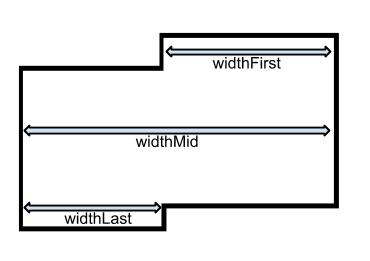
\includegraphics[scale=1.0]{Images/image03.png}
	\caption{тип Format}
\end{figure}
\\Это нововведение позволит более гибко комбинировать блоки текста и увеличит количество возможных вариантов, что позволит делать более качественный итоговый вывод. 

Кроме описания полей этого типа, возникает необходимость задать его алгебру. Для начала инициализируем операторы для данного типа. Они являются переопределенными аналогами комбинаторов типа Doc, исключая комбинатор Choice(его роль описывалась выше).

Для более четкого представления алгебры определим два формата f1 и f2 и соответствующие поля для каждого из них: first, mid, last, height. Рассмотрим изменения которые происходят с объектами Format при различных операциях.

\textit{Комбинатор Above}
\begin{figure}[h]
	\centering
	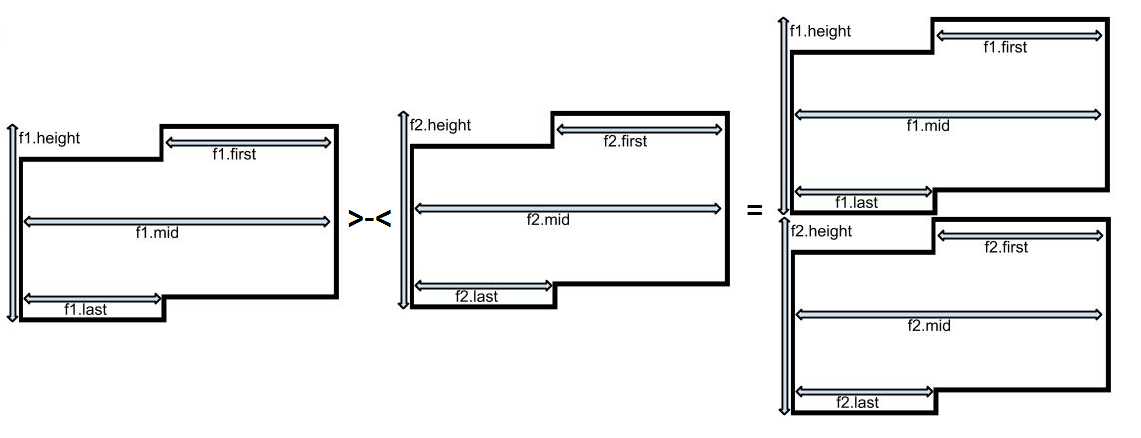
\includegraphics[scale=0.4]{Images/image02.png}
	\caption{Комбинатор Above}
\end{figure}

Новый формат будет иметь следующие параметры
\begin{lstlisting}
let newFirst = f1.first
        let newMid = 
            List.max [(if f1.height > 1 then max f1.mid f1.last  else 0); 
                      (if f2.height > 1 
                       then max f2.first f2.mid else max f1.mid f1.last);]
        let newLast = 
            if f2.last <> 0 then f2.last else f1.last
        let newHeight = f1.height + f2.height
        let newFun = fun n -> f1.txtstr n << nl_skip n << f2.txtstr n
\end{lstlisting}
%%%%%%%%

\textit{Комбинатор Beside}

\begin{figure}[h]
    \centering
	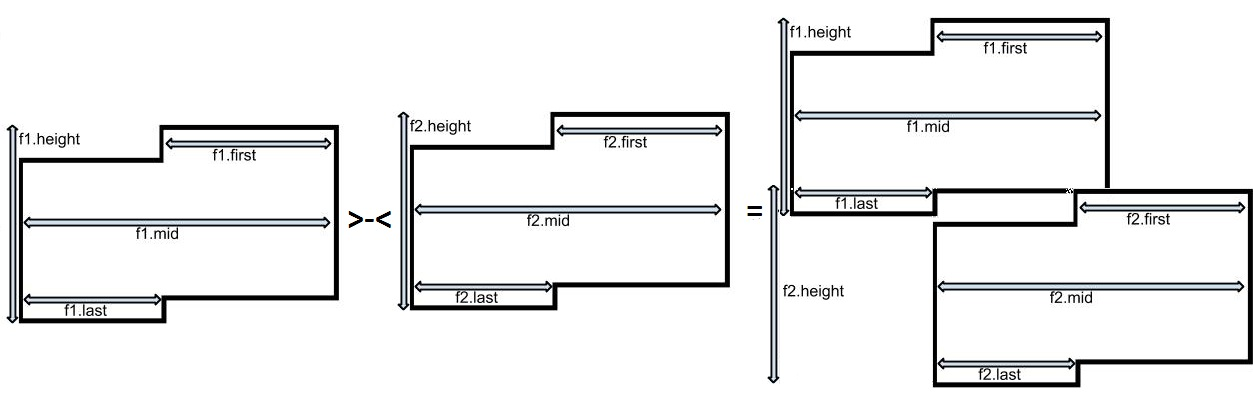
\includegraphics[scale=0.5]{Images/image07.png}
	\caption{Комбинатор Beside}
\end{figure}
\newpage

Новый формат будет иметь следующие параметры

\begin{lstlisting}
let newFirst = 
            (if f1.height <> 1 then f1.first
             else f1.first + f2.first)
        let newMid = 
            List.max [(if f1.height > 1 then f1.mid else 0); 
                      (if f1.height = 1 && f2.height = 1 then f1.mid + f2.mid else 0);
                      (if f2.height > 1 then max (f1.last + f2.first) (f1.last + f2.mid) 
                                        else f1.mid);]
        let newLast = f1.last + f2.last
        let newHeight = f1.height + f2.height - 1
        let newFun = fun n -> f1.txtstr n << f2.txtstr (f1.last + n)
\end{lstlisting}
%%%%%%%%

\textit{Комбинатор Fill}

Добавление параметра первой строки позволяет определить еще один оператор, который конкатенирует последнюю и первую строку двух форматов и и делает операцию Above с остальной частью блока. Это делает вывод красивее и позволит в будущем реализовать принтер использующий шаблоны. 

\begin{figure}[h]
	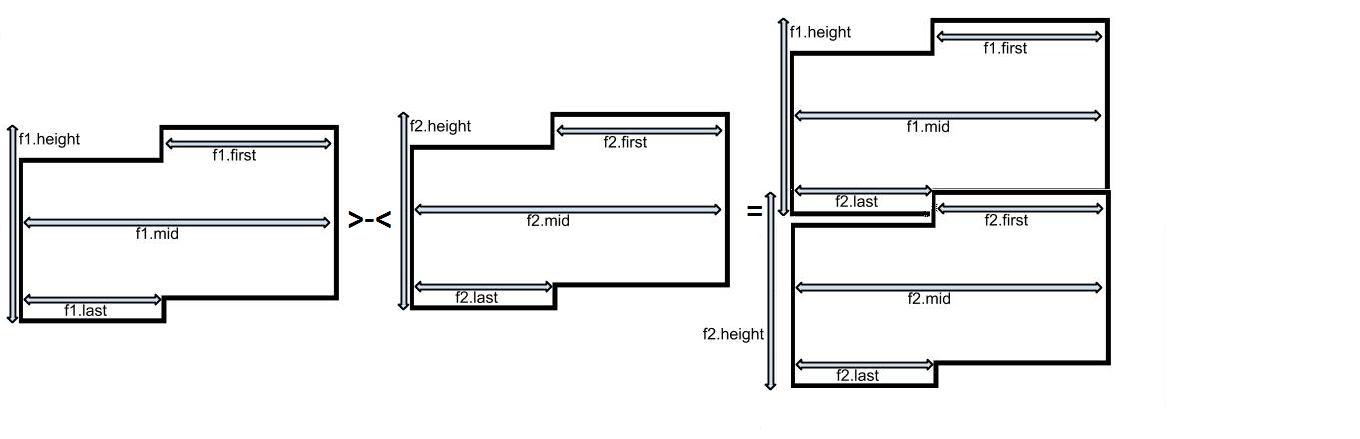
\includegraphics[scale=0.5]{Images/image12.png}
	\caption{Комбинатор Fill}
\end{figure}
\newpage

Новый формат будет иметь следующие параметры
\begin{lstlisting}
let newFirst = 
            if f1.height <> 1 then f1.first
            else f1.first + f2.first
        let newMid =
            List.max [(if f1.height = 1 && f2.height = 1 then f1.mid+f2.mid  else 0);
                      (if f1.height > 1 && f2.height = 1 then f1.mid         else 0); 
                      (if f1.height = 1 && f2.height > 1 then f2.mid + shift else 0);
                      (if f1.height > 1 && f2.height > 1 
                       then max (f1.last + f2.first) (f2.mid + shift) 
                       else 0);]
        let newLast = 
            if f2.height <> 1 then f2.last + shift
            else f1.last + f2.last
        let newHeight = f1.height + f2.height - 1
        let newFun = fun n -> f1.txtstr n << f2.txtstr (n + shift)
\end{lstlisting}
%%%%%%
\subsection{Реализация алгоритма}
Для преобразования типа Doc во множество форматов используется рекурсивная функция\begin{lstlisting}  
docToFormats :: Doc -> Dictionary<Frame, Format>\end{lstlisting}
Она сопоставляет каждому шаблону документа соответствующий ассоциативный массив и затем производит их склейку в комбинаторе choice.
Не вдаваясь в сложности реализации данной функции, чтобы получить множество \textit{всевозможных} оптимальных раскладок, необходимо на каждом уровне рекурсии производить следующие действия: 
\begin{itemize}
    \item Инициализировать новый результирующий ассоциативный массив res
    \item При наличии шаблона Text добавить в res объект типа Format содержащий текст
    \item При наличии шаблонов Indent, Above, Beside, Fill, для каждого из документов посчитать docToFormats и затем произвести прямое произведение полученных массивов используя в качестве оператора для каждой пары  соответствующий шаблону комбинатор
    \item В  шаблоне Choice склеить два массива в один
\end{itemize}
Как заметил автор библиотеки~\cite{podkopaevD} и как видно из рисунка 1 Doc на самом деле является \textit{ориентированным ациклическим графом(direct acyclic graph)}. Для уменьшения сложности алгоритма необходимо инициализировать ассоциативный массив, содержащий  посчитанные раскладки. После данной оптимизации алгоритм приобретает необходимую нам полиномиальную сложность.
Для выбора оптимального формата используется функция \begin{lstlisting} 
best :: int -> Dictionary<Frame, Format> -> Format\end{lstlisting}
\subsection{Проверка корректности}
Важным этапом в разработке стала проверка корректности работы библиотеки. Необходимо было убедиться, действительно ли алгоритм принтера выводит синтаксически и семантически правильный результат. Для этого была использована библиотека BrahmaFsharp~\cite{brahma} Выбор был обусловлен тем, что в ней имелись нужные для проверки корректности тесты и в качестве принтера уже использовалась библиотека FSharpx.Text.StructuredFormat . На данном этапе основной задачей стало создание интерфейса для обеспечения легкого перехода с библиотеки StructuredFormat. Для этого был написать отдельный модуль содержащий все основные функции StructuredFormat, но работающий на разрабатываемой библиотеке.
По завершении создания модуля, библиотека StructuredFormat была подменена на YC.PrettyPrinter в BrahmaFsharp и проведено тестирование. Результаты тестирования показали эквивалентность работы двух библиотек с точки зрения компилятора.
\subsection{Проверка оптимальности и сложности алгоритма}
Для проверки оптимальности вывода был сгенерирован ряд синтетических тестов. В качестве целевого языка выступал описанный ранее язык L. К нему были добавлены модули принтеров использующие две библиотеки. Как и в случае с проверкой корректности модули являются идентичными за исключением используемых библиотек. Для тестирования использовались сгенерированные файлы неформатированного кода на языке L. Тесты делятся на несколько категорий:
\begin{itemize}
    \item Тест работоспособности
    \item Тесты генерации вывода
    \item Тесты проверки эквивалентности кода двух библиотек.(этот блок тестов отображает разницу вывода)
    \item Тесты производительности
\end{itemize}
Важным моментом являются тесты эквивалентности и производительности. Эти два блока показывают, что на структурах с большим количеством ветвлений в документе, YC.PrettyPrinter почти совпадает с Text.StructuredFormat по скорости работы, и даёт более оптимальный вывод.

На вход тестов подавались файлы с кодом на языке L. Каждый файл содержал в себе n раз вложенные блоки if - else. Далее производились функции печати на каждой из библиотек и выполнялись замеры скорости работы на одном компьютере. Результаты замеров производительности следующие:
\begin{figure}[h]
    \centering
	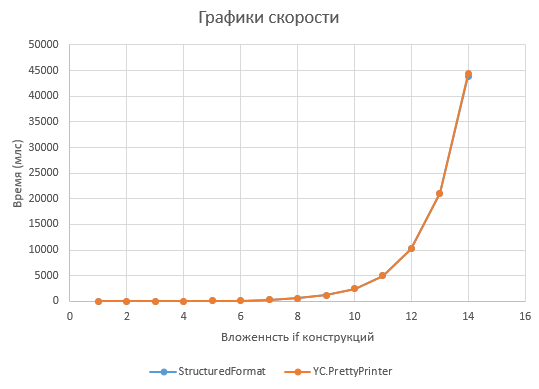
\includegraphics[scale = 1.0]{Images/diagram.PNG}
	\caption{График скорости}
\end{figure}
\begin{table}
    \centering
    \begin{tabular}{|c|c|c|}
    \hline
    N  & StructuredFormat & YC.PrettyPrinter \\ \hline
    1  & 2,557            & 2,468            \\ \hline
    2  & 6,222            & 6,261            \\ \hline
    3  & 15,382           & 14,847           \\ \hline
    4  & 31,067           & 31,773           \\ \hline
    5  & 65,63            & 67,644           \\ \hline
    6  & 144,634          & 144,048          \\ \hline
    7  & 282,333          & 283,913          \\ \hline
    8  & 577,904          & 577,17           \\ \hline
    9  & 1186,038         & 1190,98          \\ \hline
    10 & 2441,083         & 2455,089         \\ \hline
    11 & 4990,157         & 5030,768         \\ \hline
    12 & 10246,302        & 10289,875        \\ \hline
    13 & 21028,047        & 21111,7019       \\ \hline
    14 & 43916,371        & 44423,984        \\ \hline
    \end{tabular}
\end{table}
\newpage

Из них можно сделать вывод, что на большом количестве узлов библиотека \sloppy{YC.PrettyPrinter} работает незначительно медленнее чем библиотека Text.StructuredFormat.

Кроме того оптимальность вывода становится очевидна даже на минимальном дереве. На рисунке ниже приведены результаты работы обоих библиотек. В качестве требуемой ширины вывода было установлено значение 22.
\par
\begin{figure}[h]
    \centering
	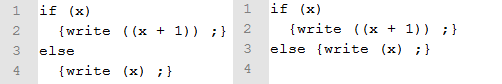
\includegraphics{Images/image00.png}
	\caption{Разница в выводе}
\end{figure}
\par
Как видно из рисунка  библиотека YC.PrettyPrinter выполнила условие оптимальности, а библиотека Text.StructuredFormat - нет.
\section{Заключение}
В рамках данной работы были достигнуты следующие результаты:
\begin{itemize}
    \item Изучен подход для построения принтеров на функциональном языке.
    \item Реализована принтер-комбинаторная библиотека на языке F\# для платформы .NET
    \item Доказано, что данная библиотека предоставляет более качественный вывод чем Text.StructuredFormat  относительно заданной ширины
    \item Реализован линейный вариант библиотеки(не дающий оптимальности), для использования её в системах в которых производительность важнее оптимальности
\end{itemize}
В качестве дальнейших направлений развития библиотеки необходимо изучить подход к заданию принтеров целевого языка с помощью шаблонов и реализовать данную методику.

prИсходный код библиотеки достпен по ссылке \sloppy\url{https://github.com/YaccConstructor/YC.PrettyPrinter}. Автор был зарегистрован под именем : AndreyBulgakov.
\bibliographystyle{ugost2008ls}
\bibliography{diploma.bib}
\end{document}
